\chapter{Trabalhos Relacionados}

Este capítulo tem como propósito destacar os estudos mais relevantes à proposta de tese e que fizeram parte do caminho percorrido para chegar na proposta final da tese.  A seção 3.1 descreve a minha atuação como professor colaborador, através do estágio docente, para alunos da graduação na disciplina, Fundamentos da Engenharia de Software da UFRJ, em 2018.  A Seção 3.2 detalha a aplicação do Protocolo Copus, desenvolvida durante o acompanhamento de aulas de matemática junto ao Instituto Superior Técnico(IST) com intuito de avaliar a motivação de estudantes. A seção 3.3 detalha a aplicação de um Escape Room também no âmbito do IST junto a estudantes do ensino superior que frequentavam as aulas de lógica de programação e matemática, também para avaliar a motivação de estudantes. Na seção 3.4, é apresentado o resultado das pesquisas relativas a quizzes aplicados em autorregulação da aprendizagem. Na seção 3.5 é apresentado o trabalho realizado junto a análise de dados de cursos da plataforma de MOOC do IST. Na seção 3.6 é detalhado o projeto criado a partir da tese e em parceria entre a UFRJ e o IST, denominado igualdade STEM. Por último, na Seção 3.7 são feitas as considerações finais do capítulo.

\section{Aulas de Fundamentos de Engenharia de Software na UFRJ}

Durante o curso, da disciplina Fundamentos da Engenharia de Software, ministrado no primeiro período de 2018, na Universidade Federal do Rio de Janeiro foram aplicados conceitos teóricos e práticos sobre a engenharia de software, bem como atividades relacionadas ao desenvolvimento colaborativo de software, entre os alunos da UFRJ \citep{github_fes-ufrj_2018}, a comunidade de software público i-Educar \citep{portal_i-educar_2009} e a prefeitura municipal de Caxias, através da secretaria municipal de educação.

Minha atuação foi como professor colaborador, através do estágio docente. Na maioria das vezes em que a disciplina é ofertada os alunos aprendem a parte da teoria, mas sem a experiência de desenvolver um software para um caso real.

Neste sentido, para cumprir os requisitos da disciplina, Fundamentos da Engenharia de Software, os alunos precisaram entregar um projeto completo de \textit{software}, passando pela especificação, desenvolvimento, validação, evolução e testes.  

O projeto teve como base um componente para a comunidade do Software Público i-Educar \citep{portal_i-educar_2009}, como entrega final da disciplina, tendo todo o processo sido documentado através de páginas wiki e o repositório da disciplina no Github \citep{github_fes-ufrj_2018}.

No primeiro mês de aula, foram analisados alguns conceitos básicos sobre Canvas, Métodos Ágeis, \textit{Scrum}, UML, a linguagem Java e seu ambiente de desenvolvimento, a Ide Netbeans e suas funcionalidades, testes e demais conceitos necessários para desenvolver o sistemas dentro deste contexto de aprendizado.

Durante todo o período letivo de aulas, os alunos tiveram a abordagem de sala de aula invertida. Durante as aulas presenciais os alunos tiveram slides de teoria sobre engenharia de software, mescladas com apresentações ao vivo, de forma remota com outros especialistas sobre assuntos diversos usando a ferramenta \textit{appear.in} \citep{apper.in_appear._2019}. 

Além disso, outras aulas presenciais contaram com apresentação de vídeos selecionados da plataforma \textit{youtube}, dinâmicas em grupos, entrevistas com clientes da prefeitura de Caxias, apresentações de outros alunos, preenchimento colaborativo de Canvas e prática do \textit{Scrum}, contendo a)planejamento, b)revisão e c)retrospectiva.

Dentre as atividades, fora da sala de aula, o \textit{HackComb} merece destaque. Durante uma greve na universidade, os alunos perderam uma aula, que foi reposta num dia de feriado, dentro de uma empresa desenvolvedora de software, denominada, Helabs. 

\textit{HackComb} - Hackeando o combustível foi o nome dado a este dia. O nome deste evento é uma adaptação em um formato bem menor de dois conceitos: \textit{Hackathon}. É também uma brincadeira com relação a falta de combustíveis em nosso país. O fato de não existir combustível nos postos, gerou uma greve da faculdade e nos possibilitou usar combustível novo em nosso projeto da disciplina. O que era uma âncora, virou vento favorável e foi o momento de aplicarmos de forma intensa nossa energia usando o tempo a nosso favor.

Durante este dia os alunos tiveram a aplicação da técnica pomodoro  e a participação remota de outros alunos que não puderem estar presentes. Todo o processo de trabalho foi documentado através de página \textit{wiki} da turma, contendo fotos e descrição das tarefas, que se encontram no repositório da turma.  

Abaixo segue a linha do tempo, bem como os conteúdos aprendidos, durante o curso:

\begin{figure}
    \centering
    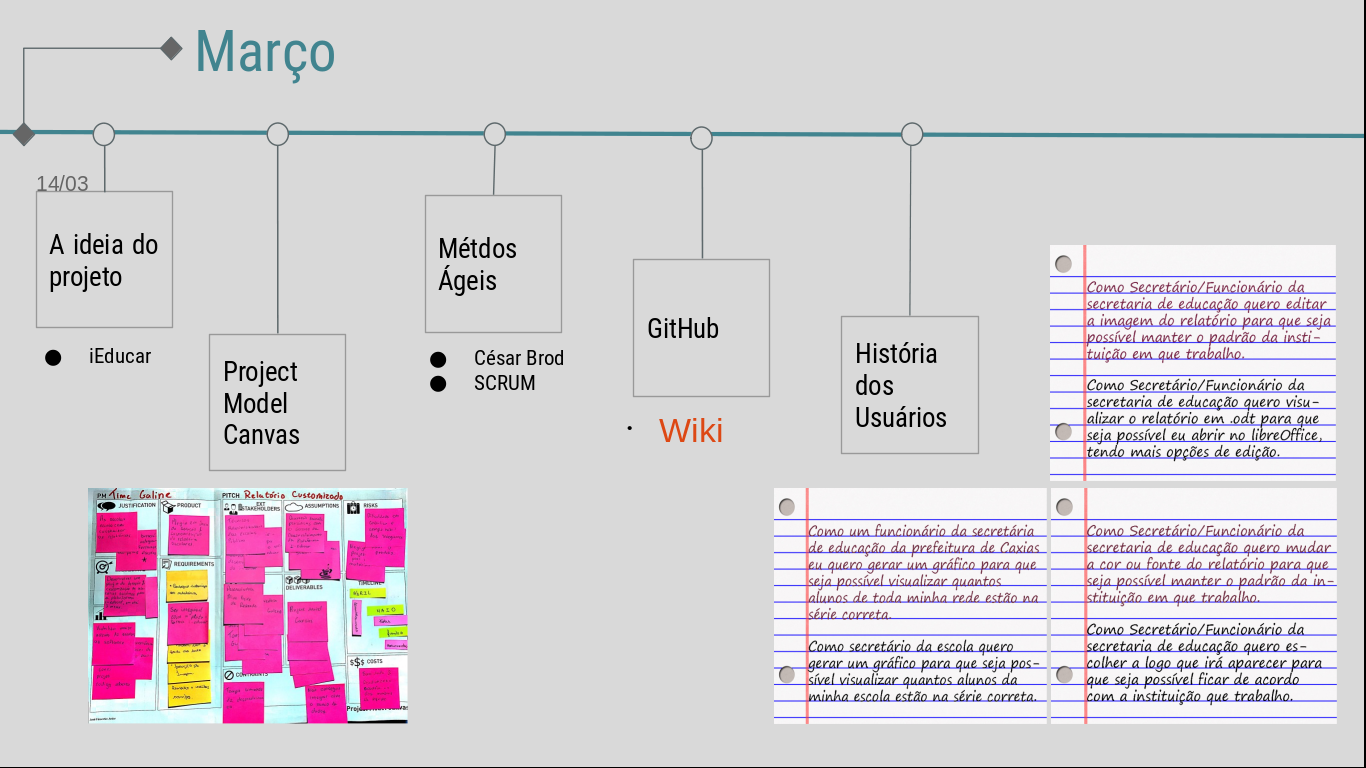
\includegraphics[width=.9\textwidth]{chaps/Images/Linha-tempo1.png}
    \caption{FES-UFRJ - Março-2018.}
    \label{fig:linha-dotempo1}
\end{figure}

\begin{figure}
    \centering
    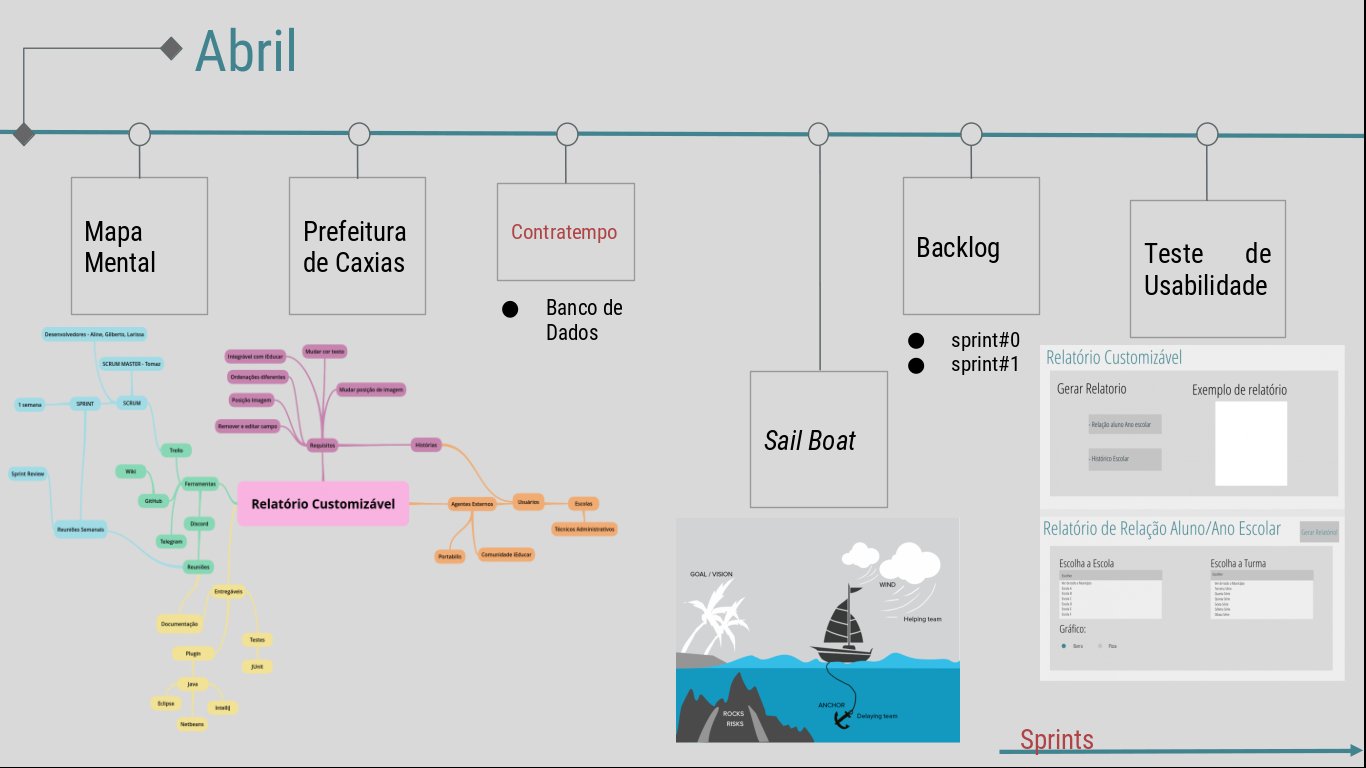
\includegraphics[width=.9\textwidth]{chaps/Images/linha-tempo2.png}
    \caption{FES-UFRJ - Abril-2018.}
    \label{fig:linha-dotempo2}
\end{figure}

\begin{figure}
    \centering
    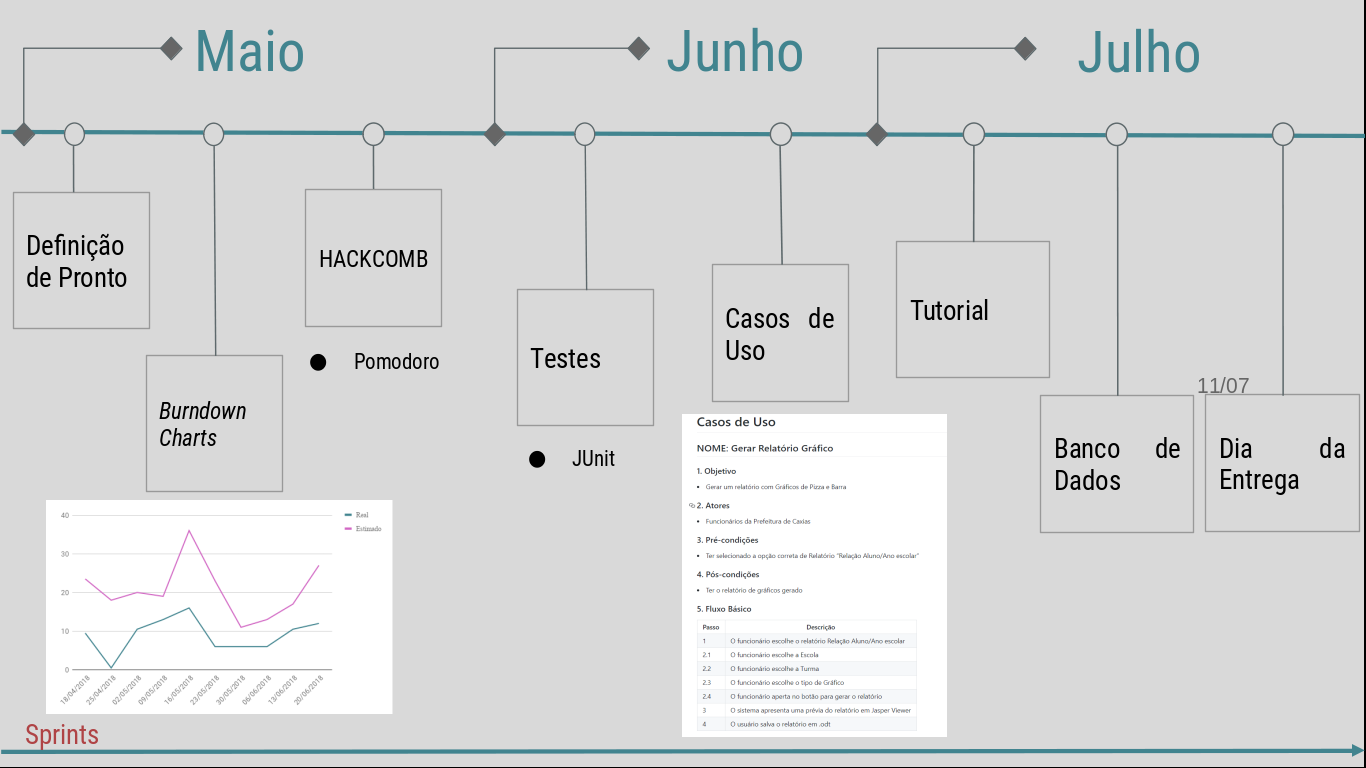
\includegraphics[width=.9\textwidth]{chaps/Images/maio.png}
    \caption{FES-UFRJ - Maio/junho/julho-2018.}
    \label{fig:linha-dotempo3}
\end{figure}


Podemos concluir que os alunos tiveram evolução nas suas habilidades com relação aos temas propostos na aula, conforme uma tabela elaborada por um dos times:

\begin{figure}
    \centering
    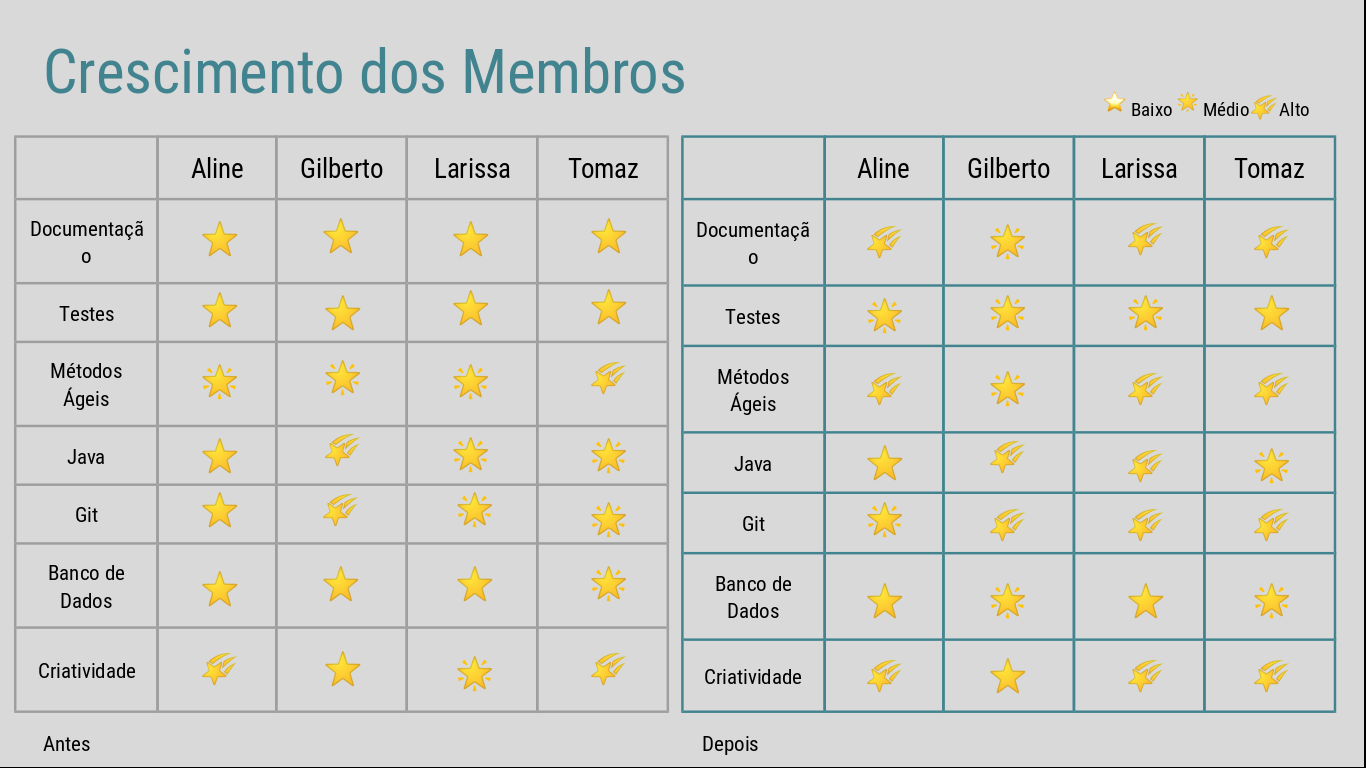
\includegraphics[width=.9\textwidth]{chaps/Images/Habilidades.png}
    \caption{FES-UFRJ - Evolução das habilidades}
    \label{fig:habilidades}
\end{figure}

Todos os times trabalharam com páginas \textit{wiki} de conteúdo aberto que permitiu uma troca de conhecimentos durante as aulas, podendo cada time ver os conteúdos produzidos pelos outros times, também foi disponibilizado um grupo no telegram para continuidade das aulas de forma virtual. Neste grupo existiam a presença de outros especialistas em assuntos diversos, como hackers, desenvolvedores, líderes de comunidades de softwares e especialistas em tecnologia. Todos os alunos compartilhavam suas dúvidas e todos ajudavam. 

Em alguns momentos foram apresentadas tarefas aleatórias com tempo de entrega, onde o primeiro aluno que realizasse a tarefa ganhava uma surpresa, que podia ser um livro, uma camisa ou uma menção honrosa.

Durante as aulas os alunos que conseguiam avançar com alguma atividade, ajudavam os outros que ainda não tinham conseguido realizar. Foram realizadas dinâmicas de meia hora entre os grupos de forma que eles pudessem discutir entre eles algum assunto escolhido para o outro grupo apresentar. Um exemplo disso eram as reuniões virtuais realizadas entre os grupos para ajuda mútua. 

\section{Aplicação do Protocolo Copus}

"Os instrutores e as práticas de ensino que eles empregam desempenham um papel fundamental na melhoria da aprendizagem dos alunos nos cursos de ciências, tecnologia, engenharia e matemática (STEM) da faculdade"(Paper Copus). Em decorrência destas constantes transformações na área da educação, é necessário coletar e analisar informações sobre o que acontece durante o tempo que decorre uma aula. Para que esta análise, principalmente sobre a motivação de estudantes, seja possível, nesta fase da pesquisa usamos um protocolo de observação em sala de aula conhecido como Protocolo de Observação em Sala de Aula para Graduação STEM ou COPUS(Citar). Este protocolo permite que o corpo docente do STEM, após um curto período de treinamento de 1,5 horas, caracterize de forma confiável como o corpo docente e os alunos estão gastando seu tempo na sala de aula(Citar). As aulas monitoradas e preenchidas com a planilha do protocolo(Citar planilha) foram as aulas regulares de Álgebra Linear, ministradas pela Professora Ana Moura Santos na graduação de informática do IST.

Os dados capturados nas observações são referentes a 15 aulas de uma mesma professora e duas outras aulas de dois professores diferentes. As análises que mostraremos abaixo se dividem em três considerando as particularidades da amostra. A primeira análise considera todas as aulas, a segunda somente as aulas da professora com maior frequência, que será nomeada aqui como Professora 1 e a terceira fixa-se somente nos dados das duas aulas dos outros dois professores.

Os dados completos foram analisados à luz de dois algoritmos de classificação baseados em árvore de decisão.
O primeiro algoritmo que foi rodado é o rpart. Por esse algoritmo chegou-se à seguinte árvore simples de decisão mostrada no Gráfico 1.


\begin{figure}
    \centering
    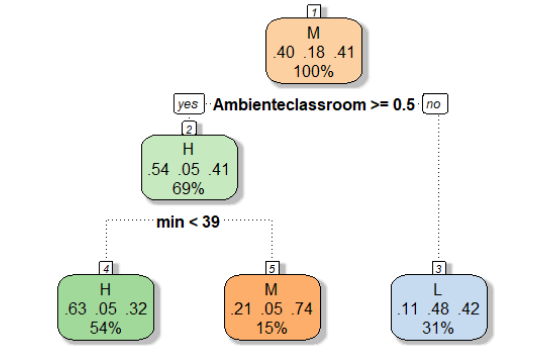
\includegraphics[width=.9\textwidth]{chaps/Images/figura1copus.png}
    \caption{Árvore simples de decisão}
    \label{fig:arvore_simples_decisao}
\end{figure}

A leitura do Gráfico 1 indica que do total das combinações de anotações 41\% são de médio engajamento, 40\% são de alto engajamento e aproximadamente 18\% de baixo engajamento.
Desse total, 31\% dos engajamentos é explicado pelo ambiente de aula ser diferente de sala de aula, ou seja, as aulas acontecem em anfiteatro. Nesses casos, temos que 31\% das combinações referem-se a baixo engajamento.
Para os 69\% restantes há um ponto de decisão referente ao tempo de aula. Até os 39 minutos de aula há uma associação de 54\% das ocorrências para alto engajamento. No caso contrário, há 15\% das associações a médio engajamento.
Temos então que as duas situações mais importantes para o modelo usado, a ponto de aparecerem na árvore de decisão, são o ambiente onde ocorre as aulas e o tempo de aula.
A opção inicial pelo uso da árvore simples deve-se principalmente pelo fato dos seus respectivos modelos serem fáceis de ser interpretados como na figura acima. Para os objetivos desse trabalho que se referem a descrever quais variáveis e quais condições mais influenciam no engajamento dos estudantes, o uso dessa abordagem para uma primeira descoberta é válido. Porém existem outras implementações de uso de árvores de decisão que são mais robustas, principalmente para fazer predições de classificação a partir de dados observados. A desvantagem dessas outras implementações relaciona-se ao fato de não gerarem modelos tão intuitivos. Para este trabalho optou-se por uso de Floresta Aleatória, uma implementação mais robusta de árvores de decisão, para identificar outras variáveis importantes que não tinham sido destacadas quando do uso de árvore simples.
Muito embora o uso de Floresta Aleatória não permita identificar os pontos de gatilho para as decisões, como ocorrem nas árvores simples, foi possível identificar duas novas condições importantes para o modelo. Veja a tabela abaixo.



Pela tabela acima, percebe-se novamente a condição de aula em sala de aula e o tempo de aula, porém agora aparece com destaque mais duas outras condições, uma relacionada a ações dos professores e outra a ação de estudantes, respectivamente FuP e OG.
A importância das quatro variáveis ou condições mais importantes levantadas pelas análises de árvores de decisão podem ficar mais claras através das análises gráficas. As figuras abaixo trazem essa evidência.
O Gráfico 2 mostra a importância do ambiente onde ocorre a aula, especificamente da condição de aula em sala de aula. É possível também perceber a importância do tempo de aula, já que é um gráfico de linha com o tempo representado no eixo horizontal


\begin{figure}
    \centering
    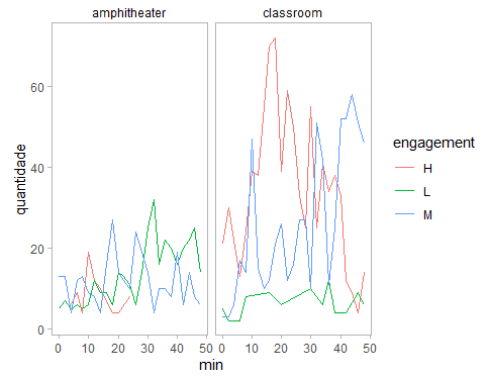
\includegraphics[width=.9\textwidth]{chaps/Images/figura2_copus.png}
    \caption{Árvore simples de decisão}
    \label{fig:arvore_simples_decisao2}
\end{figure}

\section{Aplicação de Escape Room}

\section{Mapeamento Sistemático de Autorregulação da Aprendizagem}

\section{Análise de dados no MOOC Técnico}

Neste relatório faz-se a análise de dados de três edições consecutivas dos cursos online “Controlo e Simulação de Drones” (droneX) e “Transformação Digital” (tdX), disponibilizados na Plataforma MOOC Técnico 1 . No primeiro caso, droneX, referimonos às edições de 2018, 2019 e 2020 e no segundo , tdX, considerámos as edições de 2017, 2018 e 2020. O nosso objetivo é analisar o comportamento de adesão dos 2
estudantes do Técnico Lisboa e de participantes externos inscritos nestes MOOC às atividades de avaliação, identificando padrões no seu desempenho, em particular com base no género, fazendo uma análise conhecida como Learning Analytics, Analytics e acrescentar alguns comentários individuais desses participantes enquanto avaliadores das atividades e conteúdos do droneX e do tdX. A análise com base no gênero é importante 3 no contexto da participação do MOOC Técnico no projeto
europeu FOSTWOM (2019). Este projeto tem como objetivo principal atuar na falta de equilíbrio de género nas áreas STEM, usando o potencial democrático dos MOOC.

Para a análise de dados usamos as pautas das avaliações para cada uma das edições
MOOC (em formato .csv) e fichas de perfil dos inscritos (em formato .csv), ambas
geradas pela plataforma e retiradas no final de cada edição. Incluímos ainda dados de
questionários iniciais e questionários finais. Estes últimos são respondidos via Google
Forms, mas acedidos diretamente na plataforma em cada uma das edições droneX e tdX. Como contextualização indicamos os objetivos gerais, o público alvo e a organização das atividades de avaliação, em cada um dos casos, droneX e tdX. Pontualmente, foram analisados os arquivos das pautas finais do Fénix  da UC  de “Controlo de Voo” para comparação de números de estudantes inscritos nesta UC com números totais de inscrições no MOOC droneX.

Para a análise,
escolhemos os seguintes para tratar os seguintes indicadores: taxa de Completion Rate
sucesso (Completion Rate) no MOOC em cada uma das edições sucessivas dos dois cursos online; distribuição de participantes por género em cada uma das edições; número de participantes inscritos com filiação IST; taxa de sucesso relativo por género, ou seja, participantes femininos/masculinos com sucesso entre participantes inscritos femininos/masculinos; comentários de satisfação dos participantes quanto às atividades avaliativas e quanto às expectativas iniciais sobre o MOOC (dados
qualitativos).

Na realização das análises mais estruturadas usámos RStudio, que é um software
livre de ambiente de desenvolvimento integrado para linguagem R. A linguagem R é uma linguagem de programação que permite gerar gráficos com base em cálculos estatísticos, permitindo-nos analisar dados agregados provenientes de ficheiros diferentes. É importante destacar que os números apresentados neste relatório provêm de ficheiros (.csv) diferentes, provenientes da plataforma MOOC Técnico, que foram posteriormente agregados para serem tratados no RStudio. Foram agregados em cada caso, droneX e tdX, três ficheiros tipo grade e três ficheiros tipo profile, descarregados a partir da plataforma em datas imediatamente posteriores ao final de cada edição. Numa primeira etapa, os dados agregados foram limpos, uma vez que
enrollees com registos no ficheiro grade que não existem participantes inscritos (enrollees)
estão no ficheiro profile, profile e vice-versa. A agregação feita no RStudio dos seis ficheiros de cada curso online foi feita com base nos indicadores “id”, “username”,
“email”,“ano”(by=c('id','username','email','ano')) através do comando join . Assim, o RStudio
gera relatórios finais com números totais por curso online e por ano, por género, por
Completion rates) rates global ou parcial, por exemplo, usando os dados taxas de sucesso (Completion primários que se comportam bem para os indicadores referidos. Os números gerados
pelo RStudio, e que apresentamos neste relatório, são números que se referem a
estes últimos dados primários.

\subsection{Contexto do MOOC Simulação e Controlo de Drones (droneX)}

O MOOC “Simulação e Controlo de Drones” (droneX) é aconselhado aos estudantes
inscritos na UC “Controlo de Voo” e usado durante os semestres de execução desta
UC numa estratégia de flipped-classroom
flipped-classroom. Em particular, o resultado das atividades de avaliações do MOOC contaram em cada uma das suas edições com uma
percentagem para a nota final da UC, que é uma disciplina do 3o ano do Mestrado Integrado de Engenharia Aeroespacial. Como se pode ler na página About o curso online droneX tem como objetivo analisar o funcionamento de drones multirotores e das partes que os constituem,
saber como desenvolver um simulador para analisar o seu comportamento e projetar soluções para o seu controlo automático.
As atividades de avaliação do MOOC droneX nas suas últimas três edições consistiram em um teste de avaliação de conhecimentos relativo a cada um dos quatro módulos, e um exame final, com questões de escolha múltipla e exercícios
vários, em que cada avaliação contou com 20\% para a nota final. Quando um participante atinge pelo menos 60\% de sucesso nas atividades avaliativas do curso, recebe um Honor Certificate correspondendo a um certificado de participação no curso com sucesso (sem classificação atribuída). É com base no número de certificados emitidos que se calcula a taxa de sucesso no MOOC.


\subsection{Análise dos dados de três edições}

Estiveram inscritos na edição do droneX de 2018 um total de 1258 participantes, entre os quais 424 inscreveram-se mediante autenticação Fénix com IST ID. Nesta edição, inscreveram-se 160 participantes do género feminino, dos quais 50 participantes tiveram sucesso (pelo menos 60\% de sucesso) nas atividades de avaliação do MOOC. Com relação ao género masculino, o total de participantes inscritos foi de 1088, 14 dos quais 312 participantes tiveram sucesso. O número total de participantes femininos e masculinos que terminaram com sucesso em 2018 foi de 362, o Completion rate que resulta numa taxa de sucesso (Completionrate) geral de 29\%.

Em 2019, estiveram inscritos no droneX um
total de 428 participantes, entre os quais 341
inscreveram-se com a autenticação Fénix. Deste número, 69 participantes eram do género feminino, tendo 28 participantes terminado com sucesso. Com relação ao género masculino, o total de participantes foi de 357, tendo 150 participantes terminado com sucesso. O total de participantes femininos e masculinos que tiveram sucesso foi de 178 de participantes femininos e masculinos que tiveram sucesso foi de 178, o que resulta numa Completion rate
taxa de sucesso (Completionrate) total 42\%.

Em 2020, estiveram inscritos 518 participantes,
entre os quais 458 inscreveram-se com a
autenticação Fénix. Nesta edição do droneX,
inscreveram-se 91 participantes do género
feminino das quais 53 foram as participantes
femininas que tiveram sucesso. Com relação ao
género masculino, o total de participantes foi de 420, dos quais 213 tiveram sucesso. O número de participantes femininos e masculinos que
terminaram com sucesso foi de 266, resultando
Completion rate numa taxa de sucesso (Completion rate) geral de 51\%, a mais elevada até ao momento.

\begin{figure}
    \centering
    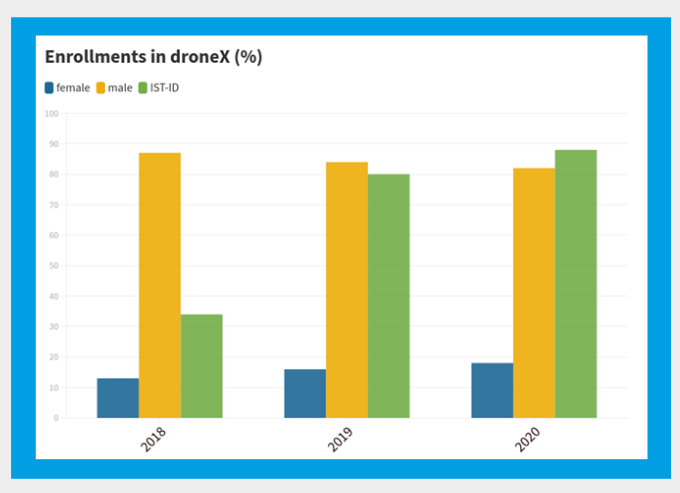
\includegraphics[width=.9\textwidth]{chaps/Images/taxa_insc_dronex.png}
    \caption{Taxas de inscrição nas várias edições do droneX}
    \label{fig:taxa_insc_dronex}
\end{figure}

Na Figura 1, podemos ver a distribuição
em cada ano da taxa de inscrição no
droneX por género (female, male) e a female, male percentagem de inscritos com filiação
IST (IST-ID), que neste caso pode indicar também estudantes inscritos na UC “Controlo de Voo” (ver ainda Fig. 5), ou alumni.

\begin{figure}
    \centering
    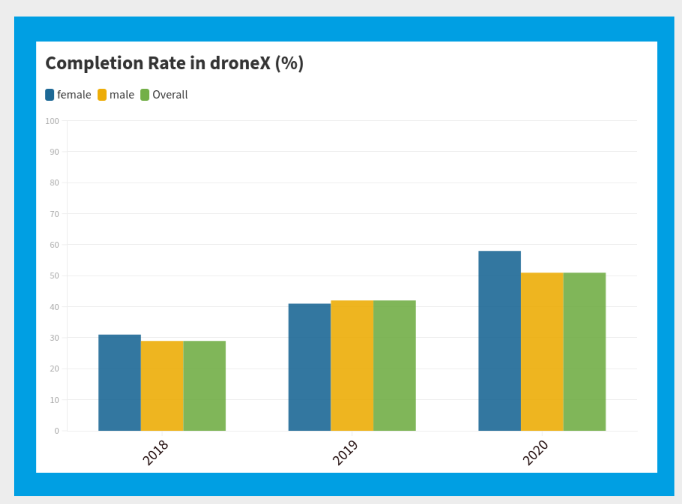
\includegraphics[width=.9\textwidth]{chaps/Images/taxa_sucesso_dronex.png}
    \caption{Taxas de sucesso nas várias edições do droneX.}
    \label{fig:taxa_sucesso_dronex}
\end{figure}

Na Figura 2, podemos ver as taxas de
sucesso (Completion rates) em cada Completion rates edição anual do droneX, percentagens
female, male género (female, female, por female, male male) e a overall percentagem total Overall A partir dos dados referidos
(Overall). acima e da visualização das duas
figuras, podemos concluir que a maioria dos inscritos no droneX são estudantes IST ou alumni do género masculino, e veremos na secção Flipped classroom com UC do Técnico  que só alguns deles são também estudantes inscritos na UC “Controlo
de Voo”.

As taxas de sucesso no droneX, exceto a total e a do género masculino na edição de 2018, situam-se acima dos 30\%. As taxas de sucesso femininas (relativas às inscrições femininas) em 2018 e 2020 ultrapassam as taxas globais.

\begin{figure}
    \centering
    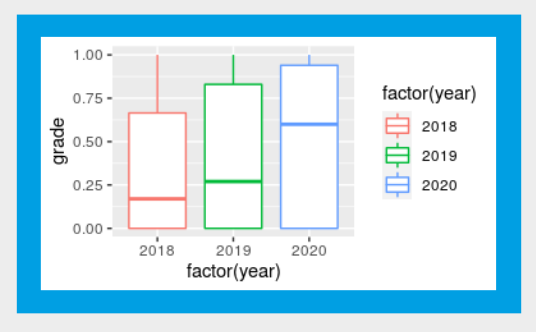
\includegraphics[width=.9\textwidth]{chaps/Images/boxplot_grade_dronex.png}
    \caption{Boxplot para a variável grade por fator year. Para cada caixa temos uma base que representa o primeiro quartil, um traço dentro da caixa que representa a mediana e o segundo quartil simultaneamente, e o topo da caixa que
representa o terceiro quartil.}
    \label{fig:boxplot_grade_dronex}
\end{figure}

No diagrama boxplot da Figura 3 podemos ver a relação entre as notas (numa escala de 0\% a 100\%) dos participantes no curso online droneX ao longo de três anos (2018, 2019 e 2020), com os dados agrupados de grade em relação ao fator year year. Verifica-se uma assimetria positiva para os dados de 2018 e 2019 e uma
assimetria negativa para os dados de 2020. É
importante notar que a mediana (segundo quartil) e o terceiro quartil das notas obtidas no MOOC tem vindo a aumentar ao longo destes três anos, estando em 2020 a
mediana próxima de 60\% e o terceiro quartil próximo dos 94\%. Recordamos que esta última edição decorreu durante um semestre académico marcado pela pandemia Covid-19, em que as aulas e a avaliação passaram para um regime remoto. O interesse e relevância de conteúdos online, em particular os MOOC, aumentaram substancialmente entre o público universitário. A caixa correspondente a 2020 é disso testemunho.

\begin{figure}
    \centering
    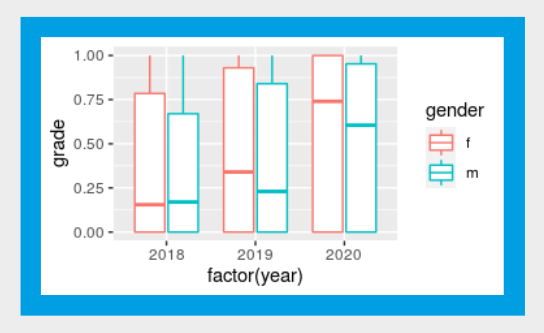
\includegraphics[width=.9\textwidth]{chaps/Images/boxplot_gender_drone.png}
    \caption{Boxplot para as variáveis grade e gender por fator year.}
    \label{fig:boxplot_gender_dronex}
\end{figure}

No diagrama boxplot da Figura 4, podemos ver a
relação entre as notas (numa escala de 0\% a
100\%) dos participantes no curso online droneX agrupados por grade e gender (f=feminino e m=masculino) em relação ao fator year (anos 2018, 2019 e 2020). Verifica-se que as assimetrias por género seguem o mesmo padrão dos dados globais, sendo positivas para os ambos os géneros em 2018 e 2019, e negativas para ambos os géneros em 2020. É importante notar que a mediana (segundo quartil) e o terceiro quartil das notas obtidas pelos participantes do droneX têm vindo a aumentar ao longo destes três anos.

Em geral, as medianas e os valores do terceiro quartil das notas de participantes femininas em 2019 e 2020 são mais elevadas do que as dos participantes masculinos. Por exemplo, em 2020 a mediana feminina encontra-se nos 74\%,
enquanto a mediana masculina está próxima de 61\%, e o terceiro quartil feminino próximo dos 100\%, enquanto o terceiro quartil masculino se encontra próximo dos 97\%. A edição de 2020 foi aquela em que houve mais participantes inscritos com sucesso nas atividades de avaliação, em particular houve muitas notas de participantes femininas próximas dos 100\%.

\subsection{Flipped classroom com
UC do Técnico Lisboa}

Para uma breve comparação entre os dados de inscrições e taxa de sucesso do droneX e da disciplina “Controlo de Voo” fornecem-se os
números abaixo. Dos participantes inscritos nas três edições referidas do MOOC droneX, um
número de 141 participantes em 2018, de 120 em 2019 e de 139 em 2020, eram também estudantes inscritos na UC “Controlo de Voo”.

De entre os 141 estudantes da UC “Controlo de Voo” de 2018, 23 estudantes eram do género feminino, dos quais 4 participantes terminaram com sucesso o droneX. Com relação ao género masculino, 119 estudantes participaram, sendo 7 os que finalizaram com sucesso.

Em 2019, o número total de estudantes inscritos na UC foi de 120. Destes, 23 estudantes eram do género feminino, e 20 destas participantes tiveram sucesso
no droneX. Com relação ao género masculino, 97
estudantes participaram, sendo 72 os que
obtiveram sucesso.

\begin{figure}
    \centering
    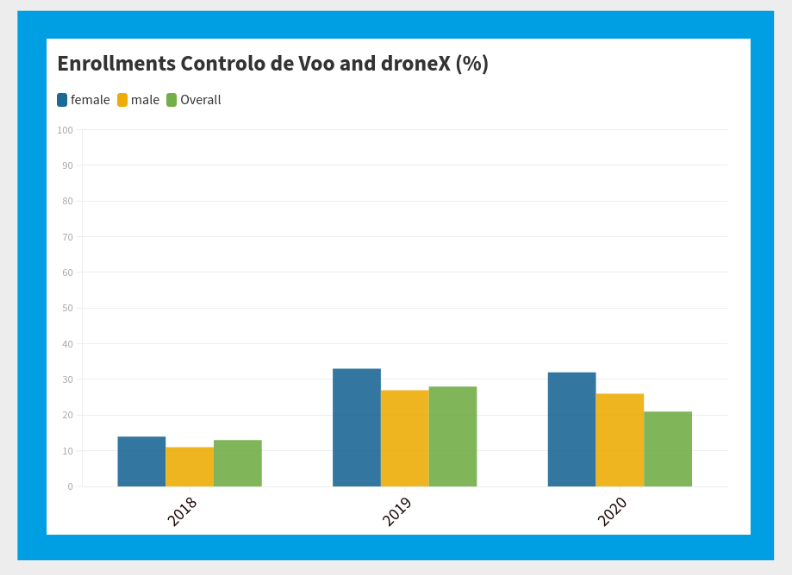
\includegraphics[width=.9\textwidth]{chaps/Images/enrollments_voo_drone.png}
    \caption{Percentagens de inscrição de estudantes da UC no droneX.}
    \label{fig:enrollment_voo_dronex}
\end{figure}

Em 2020, o número total de estudantes inscritos em “Controlo de Voo” foi de 139, dos quais 29 estudantes eram do género feminino. Destas, 27 estudantes ao participarem no droneX, obtiveram sucesso contribuindo para a
mediana próxima dos 75\% referida acima (ver
Fig. 4). Com relação aos inscritos masculinos na UC, 110 participaram no droneX, com 82 entre eles que obtiveram sucesso nas atividades de avaliação.

\subsection{Conclusão sobre a experiência global do MOOC droneX}

Podemos assim concluir que os participantes inscritos nas várias edições do droneX são estudantes IST ou 19 alumni de género masculino, mas só alguns deles são também estudantes inscritos na UC “Controlo de Voo”
(ver Fig. 5).

Relativamente à prestação feminina das várias edições do droneX, queremos sublinhar que embora exista uma percentagem baixa de alunas inscritas na UC de "Controlo de Voo” (entre 16\% e 21\%), e também de participantes femininas no MOOC (ver Fig. 1), estas
últimas alcançaram boas taxas de sucesso no droneX (ver Fig. 4). Recordamos que um dos objetivos principais do projeto europeu FOSTWOM é chamar a atenção para a falta de equilíbrio de género em muitas áreas STEM e
usar a acessibilidade dos MOOC para aumentar a
participação feminina nas áreas de Engenharia.

De modo geral, os participantes demonstraram
estar satisfeitos com as atividades de avaliação e os conhecimentos adquiridos.

Deste modo, quando se desenha e produz um MOOC a pensar em usá-lo como complemento, ou mesmo em aplicá-lo em flipped-classroom a uma UC específica do Técnico Lisboa, está a servir-se uma comunidade académica da escola mais alargada, como estudantes de outras UC e/ou alumni.

\subsection{ANÁLISE DO CURSO ONLINE TRANSFORMAÇÃO DIGITAL}

\subsection{Contexto do MOOC Transformação Digital}

O MOOC “Transformação Digital” (tdX), como se pode ler na descrição da About é aconselhado a todos os profissionais, alunos finalistas
sua página About, (prestes a entrar no mercado de trabalho) e ainda a potenciais empreendedores que tenham interesse em perceber o papel das novas tecnologias nas
organizações, tanto públicas como privadas Os participantes neste curso deverão ter interesse pelas novas tecnologias assim como vontade de transformar as organizações onde trabalham atualmente e/ou criar novos negócios.

Dentro do contexto MOOC Técnico, este MOOC é um curso online transversal para um público alargado, não obrigatoriamente académico, que tem como propósitos tirar partido das novas tecnologias para transformar as organizações, tendo como objetivo final aumentar as vendas, reduzir custos, ou criar novos negócios.

As atividades de avaliação do MOOC tdX nas suas últimas três edições consistiram em 4 exercícios de Peer Review Review. Estes exercícios são enunciados no final de cada tópico. Os participantes devem responder individualmente, sendo as respostas submetidas posteriormente avaliadas pelos seus pares, pequeno grupo de constituição aleatória de outros participantes inscritos. Finalmente, há uma revisão e confirmação da classificação mediana do grupo feitas pelo tutor.
Quando um participante atinge pelo menos 60\% de sucesso nas atividades avaliativas de Peer Review Review, recebe um Honor Certificate
Certificate, certificado de participação com sucesso (sem classificação atribuída). Recordamos que é com base no número de certificados emitidos que se calcula a taxa de sucesso no MOOC.

\subsection{Análise dos dados de três edições}

Em 2017, estiveram inscritos no tdX um total
de 1111 participantes, em que 78\% dos
participantes eram externos ao Técnico Lisboa.
Do total de participantes, 317 corresponderam a inscrições de género feminino, sendo 61 as
participantes femininas que obtiveram sucesso
(pelo menos 60\% de sucesso) nas atividades
de avaliação. Com relação ao género masculino,
21 o total de inscritos masculinos foi de 785, dos quais 162 inscritos obtiveram sucesso. O
número total de participantes que obtiveram
sucesso foi de 223, o que resulta numa taxa de
Completion Rate) geral de 20\%.

Estiveram inscritos na edição do tdX de 2018 um total de 1046 participantes, em que 73\% dos
participantes eram externos ao Técnico Lisboa.
Entre os inscritos, 336 participantes eram do
género feminino, sendo 50 as participantes que
obtiveram sucesso. O total de participantes de
género masculino foi de 707, com 137 destes
participantes a obterem sucesso nas atividades
de avaliação. O número de participantes
femininos e masculinos que obtiveram sucesso
foi de 187, o que resulta numa taxa de sucesso
Completion Rate (Completion Rate) geral de 18\%.

Em 2020, estiveram inscritos no total 1405
participantes, sendo que de novo 78\% dos
participantes eram externos ao Técnico Lisboa.
Nesta edição, 544 participantes eram do género
feminino, sendo 173 as participantes que
obtiveram sucesso. O total de participantes de
género masculino foi de 857, com 278 entre eles a obterem sucesso nas atividades de avaliação. O número de participantes femininos e masculinos que obtiveram sucesso foi de 451, o que resulta Completion Rate numa taxa de sucesso (Completion Rate) geral de 32\% que se aproxima da taxa de sucesso média de um curso MOOC Técnico.

\begin{figure}
    \centering
    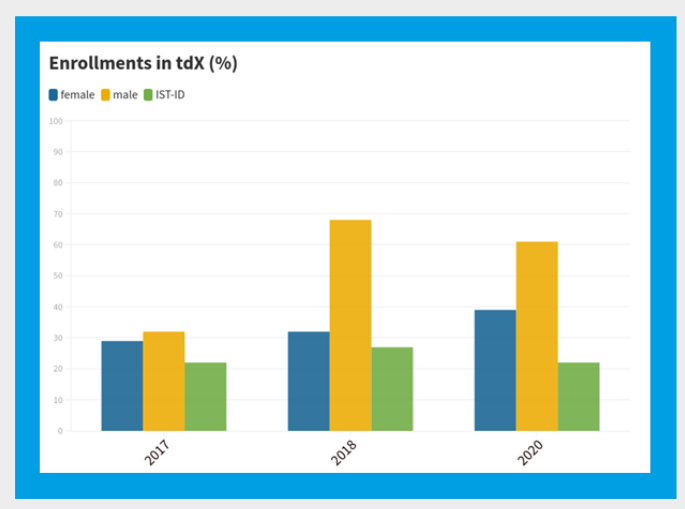
\includegraphics[width=.9\textwidth]{chaps/Images/enrollments_tdx.png}
    \caption{Taxas de inscrição nas várias edições do tdX.}
    \label{fig:enrollment_tdx}
\end{figure}

Na Figura 6, podemos ver a distribuição em cada ano da taxa de female, inscrição no tdX por género (female, male male) e a percentagem de inscritos com filiação IST (IST-ID), que neste caso é bastante inferior à percentagem
dos restantes inscritos, e bastante inferior aos valores das percentagens de inscrições com filiação IST no curso online droneX (ver Fig. 1 para os anos 2019 e 2020).

\begin{figure}
    \centering
    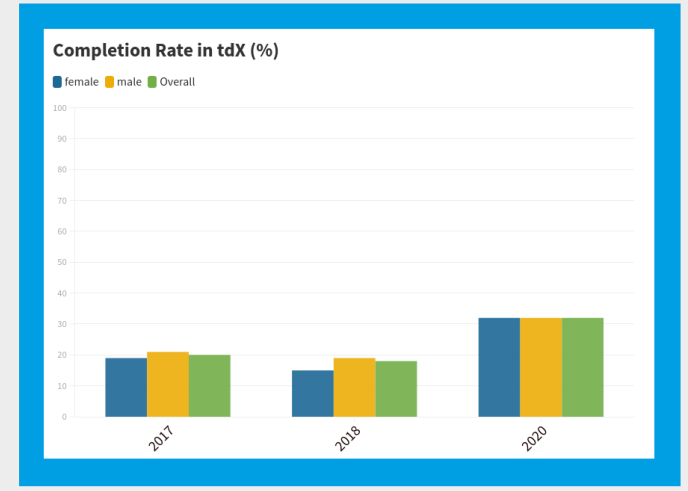
\includegraphics[width=.9\textwidth]{chaps/Images/completion_rate_tdx.png}
    \caption{Taxas de sucesso nas várias edições do tdX.}
    \label{fig:rate_tdx}
\end{figure}

Na Figura 7, podemos ver as taxas de sucesso (Completion rates) em cada Completion rates edição anual do tdX,as percentagens female, male género (female, female, por female, male male) e a overall percentagem Overall A partir dos dados total (Overall). referidos acima e da visualização das duas últimas figuras, podemos concluir que a maioria dos inscritos
no tdX são participantes externos ao IST de género masculino. As taxas de sucesso no tdX situam-se entre os 18\% e os 32\%, sendo que na última edição de 2020, todas as taxas de Overall female, male sucesso (Overall,
male) são iguais a este valor máximo de 32\%.

\begin{figure}
    \centering
    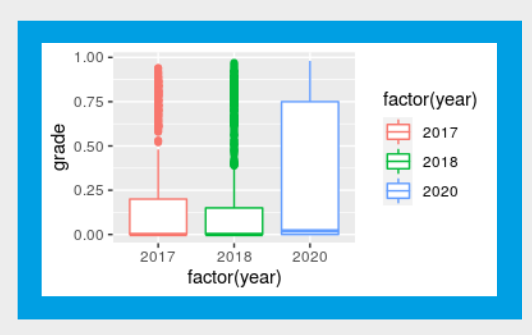
\includegraphics[width=.9\textwidth]{chaps/Images/boxplot_grade_tdx.png}
    \caption{Boxplot para a variável grade por fator year. Para cada caixa temos uma base que representa o primeiro quartil, um traço dentro da caixa que representa a mediana e o segundo quartil simultaneamente, e o topo da caixa que
representa o terceiro quartil. Os pontos isolados correspondentes às caixas vermelha e verde são outliers.}
    \label{fig:boxplot_grade_tdx}
\end{figure}

No diagrama boxplot da Figura 8, onde se pode ter uma leitura mais fina das taxas de sucesso relativas às notas obtidas pelos participantes, pode ver-se a existência de
muitos outliers outliers, principalmente nas duas primeiras edições 2017 e 2018 do tdX. Torna-se mesmo difícil de ler a mediana para esses dois anos, assim como a mediana
de 2020 que também está próxima de 2\% (numa escala de 0\% a 100\%) conferindo uma acentuada assimetria positiva nessas duas caixas. As caudas de distribuição, ou seja, as distâncias entre o terceiro quartil e o último
outlier, das notas para 2017 e 2018 também são grandes.

É importante recordar que a taxa de sucesso (Completion embora as referidas medianas se situem em valores muito baixos. Pode acontecer que o Peer Review resulte mais penalizante do que o tipo de avaliação usado no droneX. Na caixa respeitante à edição 2020 já não se visualizam outliers, outliers embora a dispersão das notas seja grande e o terceiro quartil fique nos 75\%. Recordamos que a última edição decorreu durante um período marcado pela pandemia Covid-19, em que o interesse e relevância de conteúdos online, em particular os MOOC, aumentaram substancialmente entre o público em geral. Os números de retenção desta edição 2020 do tdX
testemunham esta tendência.

\begin{figure}
    \centering
    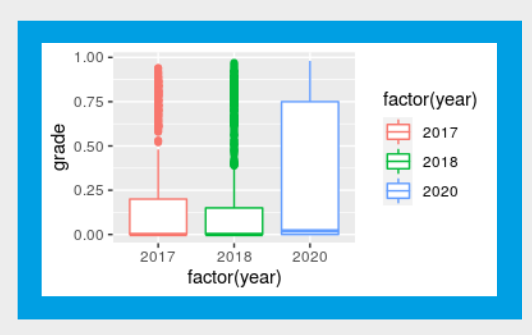
\includegraphics[width=.9\textwidth]{chaps/Images/boxplot_grade_tdx.png}
    \caption{Boxplot para as variáveis grade e gender poryear fator year.}
    \label{fig:boxplot_gender_tdx}
\end{figure}

No diagrama boxplot da Figura 9, verifica-se uma assimetria positiva muito acentuada dos dados de grade e gender (f=feminino e m= masculino) em relação ao fator year (anos 2017, 2018 e 2020) do curso online de tdX, principalmente nas caixas correspondentes às notas de participantes femininas. É possível ver com base na distribuição por género
das notas (numa escala de 0\% a 100\%) dos
participantes femininos e masculinos inscritos no tdX ao longo desses três anos, que as medianas se situam muito próximo dos 0\% em ambos os casos, sendo que na edição 2020 a mediana das notas dos participantes masculinos é próxima de 3\%.

A edição de 2020 foi aquela em que houve mais participantes inscritos que terminaram com sucesso as atividades de avaliação, em que o terceiro quartil das notas para o género masculino é de cerca de 75\%, igual ao valor do terceiro quartil global desta edição (ver Fig. 8).

\subsection{Conclusão sobre a experiência global do MOOC tdX}

Finalmente, concluímos que a maioria dos inscritos nas várias edições do tdX são participantes externos ao IST de género masculino.

Relativamente à prestação feminina nas várias edições do tdX , notamos que existe uma percentagem ligeiramente mais baixa de participantes femininas com sucesso no
MOOC (ver Fig. 7), excepto em 2020, em que a taxa de sucesso é igual para ambos os géneros. Eventualmente para esta tipologia de MOOC extracurricular faz mais sentido fazer outro tipo de análise com base noutros indicadores.

De modo geral, o público alargado, não obrigatoriamente académico, inscrito nas várias edições do curso online demonstrou estar satisfeito com as atividades de avaliação Peer Review), Review bem como com os conhecimentos adquiridos durante o curso.

Fica aqui a recomendação para se estudarem estratégias de captação e retenção de um público externo à escola, aplicando metodologias ativas que ajudem a aumentar as
taxas de sucesso nesta tipologia de MOOC transversal, com a ressalva que estas estratégias dependem muito do tópico
escolhido para o curso online, obviamente.

\subsection{Conclusão final das análises dos dados}

Terminada a análise separada sobre os dois MOOC com características distintas: o
curso “Simulação e Controlo de Drones”, droneX, dirigido principalmente a um
público de perfil “estudante IST”, e o curso “Transformação Digital”, tdX, dirigido a
um público alargado, conclui-se que a adesão às atividades de avaliação, enquanto
indicador do comportamento de adesão dos participantes a cada um dos tipos de
MOOC é também bastante distinta. Enquanto o droneX, aconselhado aos estudantes inscritos numa UC do Técnico Lisboa e usado para apoiar uma estratégia de flipped-classroom
flipped-classroom, consegue ter uma taxa média de sucesso na ordem dos 41\%, o curso “Transformação Digital”, dirigido a um público menos académico, eventualmente profissionais e potenciais empreendedores, tem uma taxa
média de sucesso de 23\%.

De referir que enquanto o número de inscritos no tdX foi sempre superior a mil inscritos, com uma maioria de inscritos externos ao IST, no droneX só na primeira edição de 2018 o número de inscritos foi superior a mil
participantes. 

Gostaríamos de acrescentar que a divulgação das várias edições do tdX beneficiaram de alguns apoios externos, enquanto no caso do droneX a divulgação foi mais interna ao IST, exceto na edição de 2018.

O público de ambos os MOOCs é predominantemente masculino (ver Fig. 1 e 6), com uma forte assimetria no caso do
droneX. Os inscritos no droneX, sendo alguns deles estudantes inscritos na UC “Controlo de Voo” (ver Fig. 5), são maioritariamente do género masculino. No entanto, as taxas de sucesso relativas (Fig. 2) e as notas obtidas (Fig. 4) pelas participantes femininas nas edições do droneX são em média superiores quando comparadas com as dos seus colegas masculinos. No caso do tdX, embora não sendo uma tendência muito acentuada, o comportamento global é o inverso (ver Fig. 7 e 9).

De modo geral, os participantes inquiridos no final de cada edição demonstraram estar satisfeitos com as atividades de avaliação e os conhecimentos adquiridos em ambos os casos, droneX e tdX (secções 2.3 e 3.3). Recordamos ainda que as últimas edições de ambos os cursos que ocorreram respetivamente, em abril e maio de 2020, durante um
Completion Rates período marcado pela pandemia Covid-19, não só tiveram taxas de sucesso (Completion Rates) mais elevadas (Fig. 2 e
7), como em geral as notas obtidas pelos participantes que terminaram com sucesso foram mais altas (Fig. 3 e 8). A apetência por este tipo de conteúdos validados, com boa qualidade gráfica, possibilitando uma formação gratuita e de fácil acesso deverá ainda aumentar nos próximos tempos.

Finalmente, gostaríamos de comentar com base nos resultados da nossa análise que um curso MOOC Técnico desenhado para um público com perfil “estudante IST de uma dada UC”, como o droneX, consegue captar e servir ainda uma comunidade mais alargada, como estudantes de outras UC, estudantes internacionais e/ou alumni que procuram aprofundar, rever ou alargar os seus conhecimentos sobre o tópico. Enquanto isso, um curso transversal,
como o tdX, para além do público externo ao IST, não obrigatoriamente académico, consegue também oferecer gratuitamente à comunidade da escola conteúdos extracurriculares de qualidade.

\section{O Projeto IgualdadeStem}

\subsection{Dados analisados}

\subsection{Evento Jornada das Mulheres}

\subsection{Artigos publicados}

\subsection{Trabalhos apresentados}





